%File: formatting-instruction.tex
\documentclass[letterpaper]{article}

\usepackage{aaai}
\usepackage{times}
\usepackage{helvet}
\usepackage{courier}
\usepackage[inline]{enumitem}
\usepackage{graphicx}
\usepackage{caption}
\usepackage{subcaption}
\usepackage{refstyle}
\usepackage{biblatex}
\addbibresource{ref.bib}
\graphicspath{ {./images/} }
\frenchspacing
\setlength{\pdfpagewidth}{8.5in}
\setlength{\pdfpageheight}{11in}
\pdfinfo{
/Title (Insert Your Title Here)
/Author (Put All Your Authors Here, Separated by Commas)}
\setcounter{secnumdepth}{0}  
 \begin{document}
% The file aaai.sty is the style file for AAAI Press 
% proceedings, working notes, and technical reports.
%
\title{ Mini-Project Report \\Sensitive Regions for Black-Box Adversarial Attacks }
\author{Sowrya Gali\\
B.Tech 3\textsuperscript{rd} Year\\
Computer Science and Engineering\\
Indian Institute of Technology, Hyderabad\\
}
\maketitle
\begin{abstract}
\begin{quote}
\emph{Deep neural networks are known to be vulnerable to adversarial attacks. Most of the emphasis, in adversarial attacks, has been on image data. The study on adversarial attacks for videos has started recently, and much work has been done in the area of White-Box attacks. In this project, we tried to visualize the saliency heat maps for YOLOv3 model, which aids in developing adversarial attacks on datasets like MS-COCO, ImageNet, etc.}
\end{quote}
\end{abstract}

\section{Introduction}
The Convolutional Neural Networks are susceptible to adversarial attacks i.e., a cleverly crafted noise is added to the image so that the network is fooled and misclassifies it. These adversarial attacks can be broadly classified into two types :  (i) White-Box Attacks and (ii) Black-Box Attacks. In white box attacks, one has access to the model architecture, dataset used by it, weights of the model etc. and using this information adversarial noise is generated. Whereas in Black-Box attacks, one usually has no access to model's parameters and hence uses a substitute model locally to craft examples by performing White-Box attacks on the local model.\\
Ever since adversarial attacks were proposed, much emphasis has been on image data and numerous attacking strategies and defense techniques were developed focusing on the image data. The study of attacks and defenses for video data and autonomous driving has been started recently.\\
In this project, we aim to detect key regions in an image that are responsible for classification and localization, so that we can perform attacks, using this information, on the dataset to fool robust models like YOLOv3\textsuperscript{\cite{redmon2018yolov3}}. Most of the works in this area are focused on developing techniques generating perturbations for general CNN architectures and they cannot perform well on robust architectures like YOLO, Faster-RCNN\textsuperscript{\cite{ren2016faster}}, SSD\textsuperscript{\cite{Liu_2016}}, etc.\ evident from \figref{PGD-YOLO}.\\
\begin{figure}[bhpt]
    \begin{subfigure}{0.93\textwidth}
        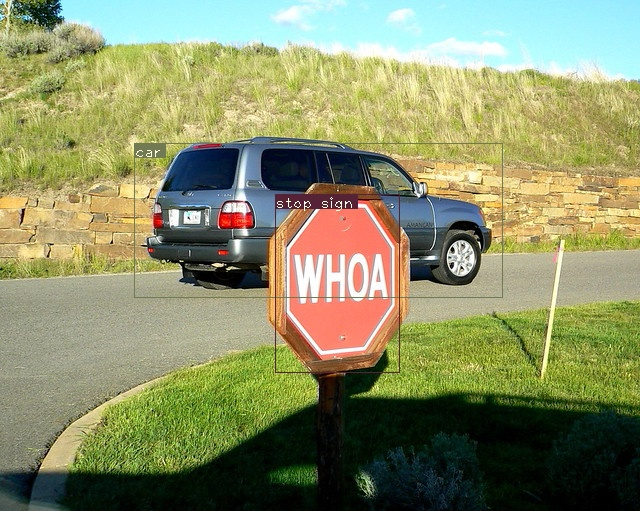
\includegraphics[width = 0.25\textwidth, height = 0.3\textwidth]{Images/yolo_det_test3.jpg} 
        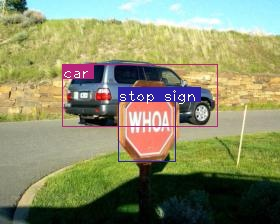
\includegraphics[width = 0.25\textwidth,  height = 0.3\textwidth]{Images/yolo_det_att.jpg}
    \end{subfigure}
    \begin{subfigure}{0.93\textwidth}
        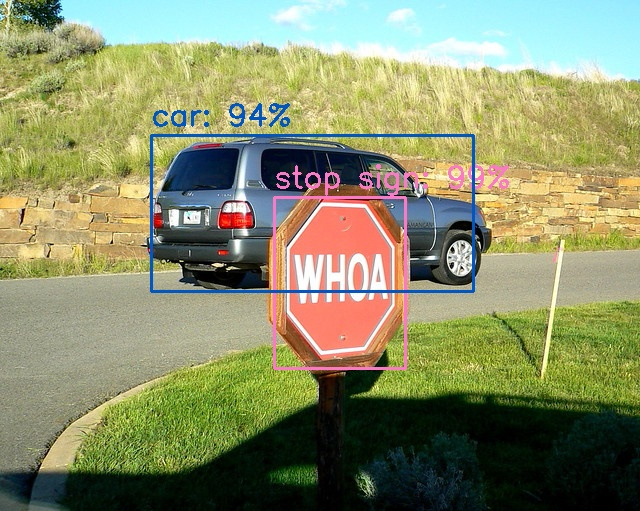
\includegraphics[width = 0.25\textwidth, height = 0.3\textwidth]{Images/FRCNN_Box_test3.jpg}
        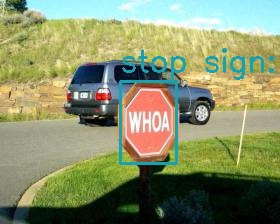
\includegraphics[width = 0.25\textwidth, height = 0.3\textwidth]{Images/FRCNN_Box_att_test3.jpg}
    \end{subfigure}
    \begin{subfigure}{0.93\textwidth}
        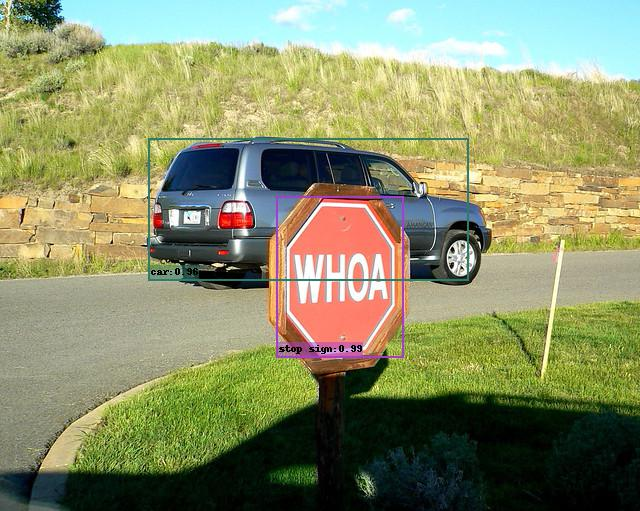
\includegraphics[width = 0.25\textwidth, height = 0.3\textwidth]{Images/ssd_test3.jpg}
        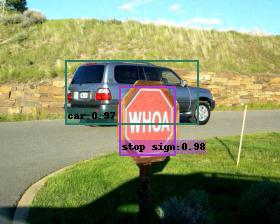
\includegraphics[width = 0.25\textwidth, height = 0.3\textwidth]{Images/ssd_att_test3.jpg}
    \end{subfigure}
    \caption{\emph{Top to bottom: Predictions of YOLOv3, faster-RCNN, and SSD on original image(left) and attacked image(right). The PGD attack is used to craft the adversarial samples using ResNet-51 as surrogate network.}}
    \label{fig:PGD-YOLO}
\end{figure}
\begin{figure*}[h]
    \centering
    \begin{subfigure}{\textwidth}
        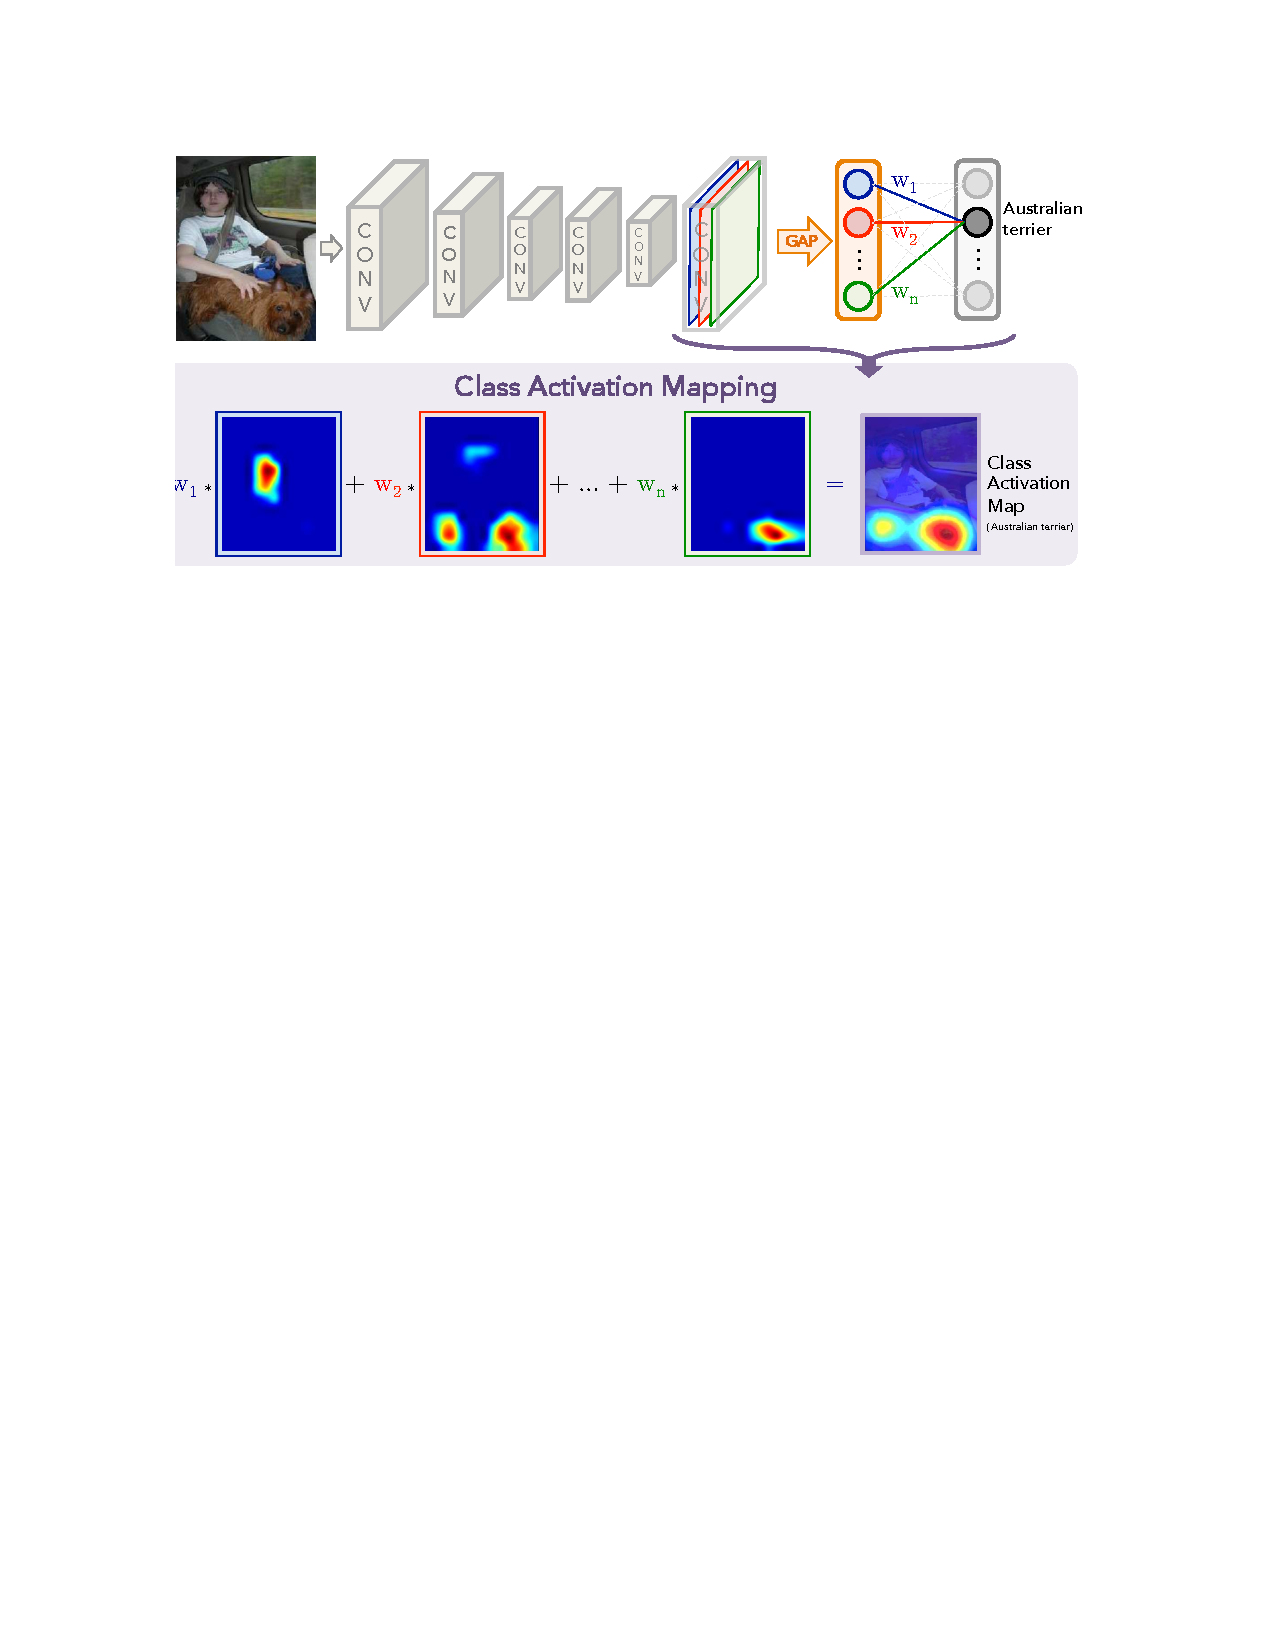
\includegraphics{Images/CAm_pic.pdf}
    \end{subfigure}
    \caption{Schematic visualization of CAM model showing how scores are mapped back from GAP layer.\cite{zhou2015learning} }
    \label{fig:CAM}
\end{figure*}
So to attack datasets, in order to fool such robust architectures, needs more investigation into the regions which activate neurons for the detection of object and it's class. Many visualization techniques have been proposed to detect feature maps for general CNNs and of these, GradCAM++ is considered to be state-of-the-art.\\
But GradCAM++, and it's predecessors are designed keeping in mind of general convolutions networks like VGG-16. Though produce good visualizations with excellent localization capabilities, there primarily based on convolutional architectures and there is no straight forward way to generalize them to non-trivial models like YOLOv3.\\
In this project, we explore possible ways of extending GradCAM++\textsuperscript{\cite{Chattopadhay_2018}}, to non-trivial architectures and how to utilize this information to perform attack on the dataset.

\section{Prior Work}
A lot of work has been done in the area of adversarial attacks and defense techniques. \cite{szegedy2014going} made the intriguing discovery of adversarial example's misclassification. Later many approaches have been proposed to create adversarial samples, \cite{goodfellow2015explaining} proposed FGSM, \cite{madry2019deep} proposed PGD attack, \cite{guo2019simple} proposed SimBA attack etc. \\
Recently, more advanced attack strategies have been proposed like \cite{jia2019enhancing} \cite{rahmati2020geoda} \cite{shi2019curls} \cite{xiao2019generating} \cite{duan2020adversarial}.\\
Ever since neural networks became popular, many efforts have been made to understand how these black-box models work under the hood. \cite{zeiler2013visualizing} made one of the first attempts in this regard. \cite{zhou2015learning} followed up with a novel approach of using Global Average Pooling(GAP) values as the saliency maps with each channel having weight same as that of it's counter part in the adjacent flattened layer, shown in \figref{CAM}. Later, \cite{Selvaraju_2019} came up with GradCAM model, which utilizes class conditional probabilities fused with pixel-based gradient visualization techniques like Deconvolution\textsuperscript{\cite{zeiler2013visualizing}} and Guided Backpropagation (GBP)\textsuperscript{\cite{springenberg2015striving}} to generate finer Heat Maps that generalize well non-GAP architectures. \cite{Chattopadhay_2018} came up with an improved version of GradCAM, called GradCAM++, which shows good localization properties on multi-object images and it is considered as one of the \emph{state-of-the-art} visualization techniques for general CNN architectures.

\section{Experimental Details}
We first started to assess  how a simple PGD attack on MS-COCO dataset could affect performance of YOLO\emph{v3}. The results of this experiment are shown in \figref{PGD-on-MS-COCO}. As evident from results, YOLO\emph{v3} is robust against these attacks. Hence we need to look into which parts of the image are responsible for predictions the model to localize attacks to these regions, and which results in better attack success rate.\\
\begin{figure*}[h]
    \begin{subfigure}{\textwidth}
        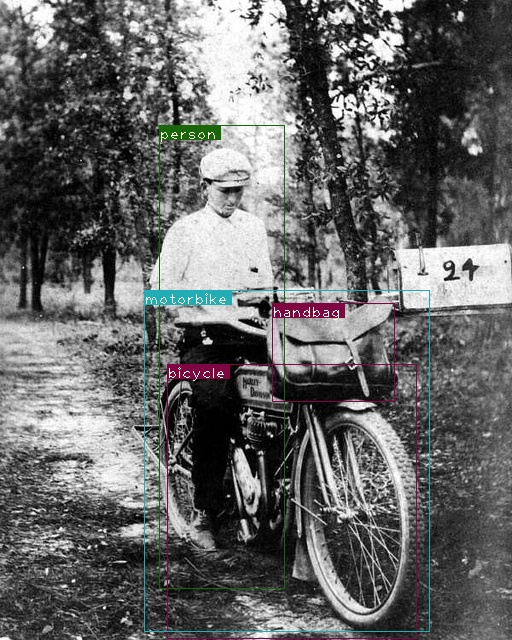
\includegraphics[width = 0.19\textwidth, height = 0.25\textwidth]{Images/Yolo-MS-COCO-original/det_test1.jpg}
        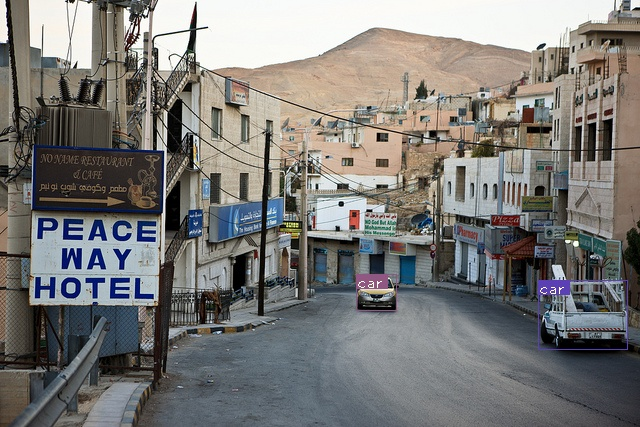
\includegraphics[width = 0.19\textwidth, height = 0.25\textwidth]{Images/Yolo-MS-COCO-original/det_test2.jpg}
        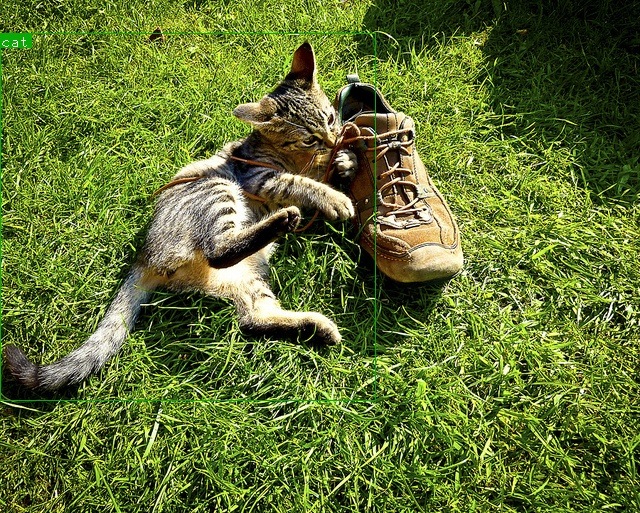
\includegraphics[width = 0.19\textwidth, height = 0.25\textwidth]{Images/Yolo-MS-COCO-original/det_test3.jpg}
        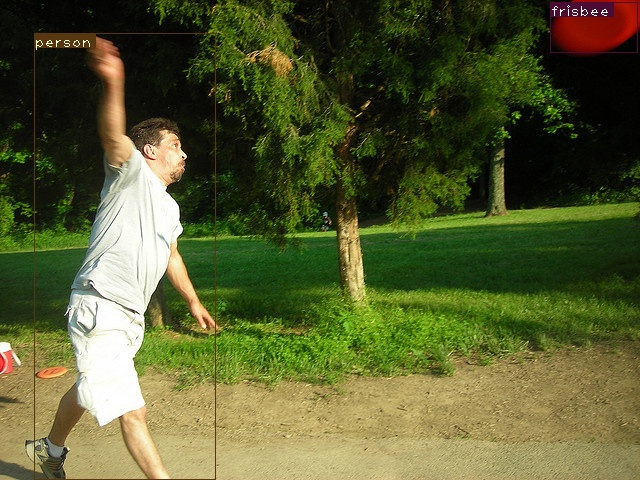
\includegraphics[width = 0.19\textwidth, height = 0.25\textwidth]{Images/Yolo-MS-COCO-original/det_test4.jpg}
        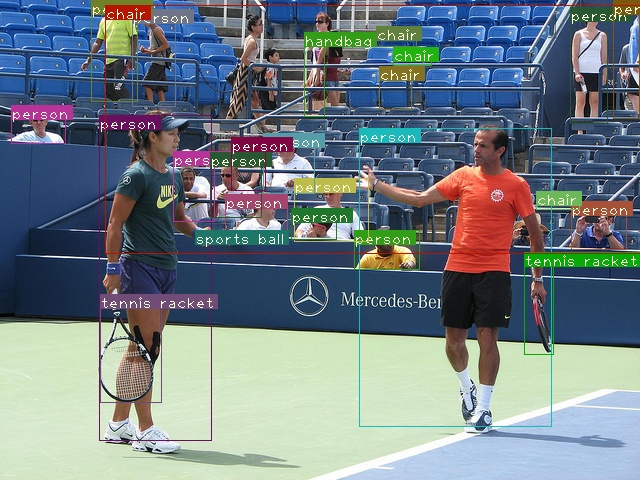
\includegraphics[width = 0.19\textwidth, height = 0.25\textwidth]{Images/Yolo-MS-COCO-original/det_test5.jpg}
    \end{subfigure}
    \begin{subfigure}{\textwidth}
        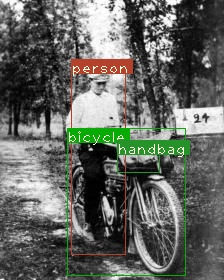
\includegraphics[width = 0.19\textwidth, height = 0.25\textwidth]{Images/Yolo-MS-COCO-Attacked/det_att_test1.jpg}
        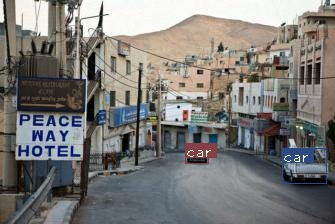
\includegraphics[width = 0.19\textwidth, height = 0.25\textwidth]{Images/Yolo-MS-COCO-Attacked/det_att_test2.jpg}
        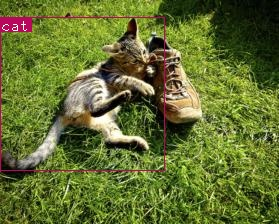
\includegraphics[width = 0.19\textwidth, height = 0.25\textwidth]{Images/Yolo-MS-COCO-Attacked/det_att_test3.jpg}
        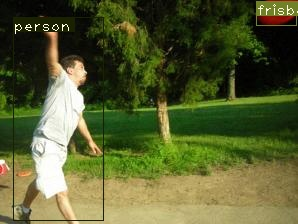
\includegraphics[width = 0.19\textwidth, height = 0.25\textwidth]{Images/Yolo-MS-COCO-Attacked/det_att_test4.jpg}
        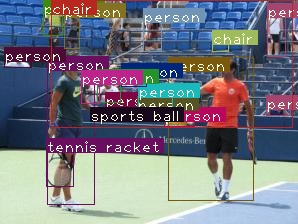
\includegraphics[width = 0.19\textwidth, height = 0.25\textwidth]{Images/Yolo-MS-COCO-Attacked/det_att_test5.jpg}
    \end{subfigure}
    \caption{A simple PGD attack is performed on some examples from MS-COCO dataset using ResNet-51 as a surrogate model. The YOLO\emph{v3} is quite resistent to this simple attacks owing to its highly complex architecture.}
    \label{fig:PGD-on-MS-COCO}
\end{figure*}
To understand the failure of PGD attack, we contrasted GradCAM++ generated heat maps of original image and attacked image. As it is evident, the attack could only slightly disperse regions of heat and there is no change especially in multi-object case as shown in \figref{heat-PGD}.\\
\begin{figure*}[h]
    \begin{subfigure}{\textwidth}
        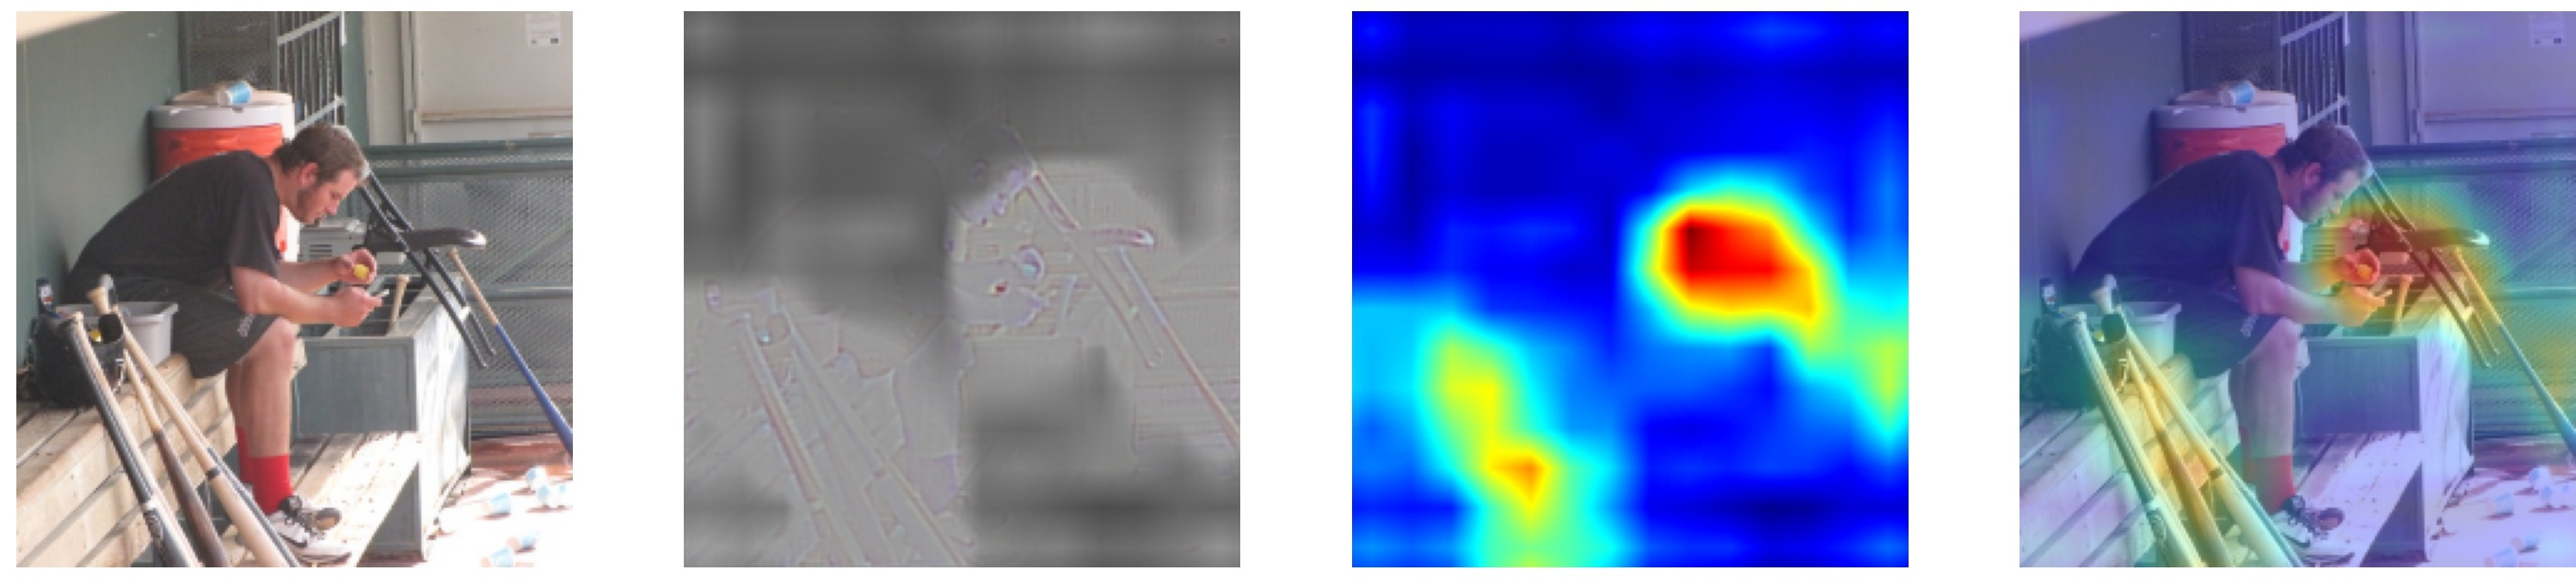
\includegraphics[width = \textwidth, height = 0.15\textwidth]{Images/HeatMapsPGD/out_test1.jpg}
    \end{subfigure}
    \begin{subfigure}{\textwidth}
        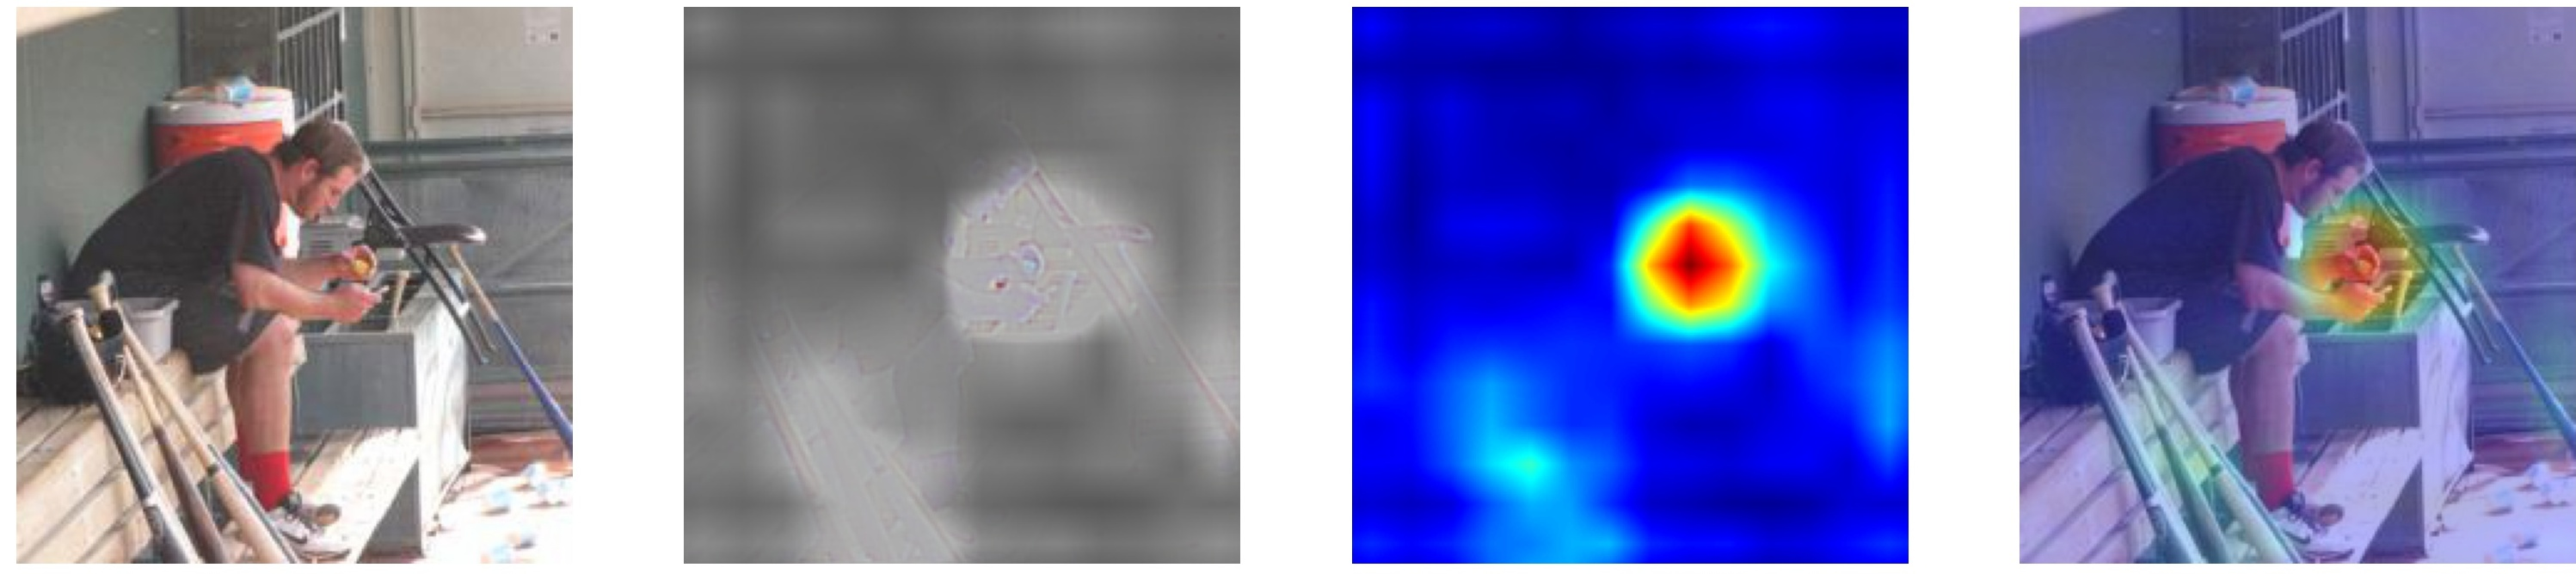
\includegraphics[width = \textwidth, height = 0.15\textwidth]{Images/HeatMapsPGD/out_att_test1.jpg}
    \end{subfigure}
    \begin{subfigure}{\textwidth}
        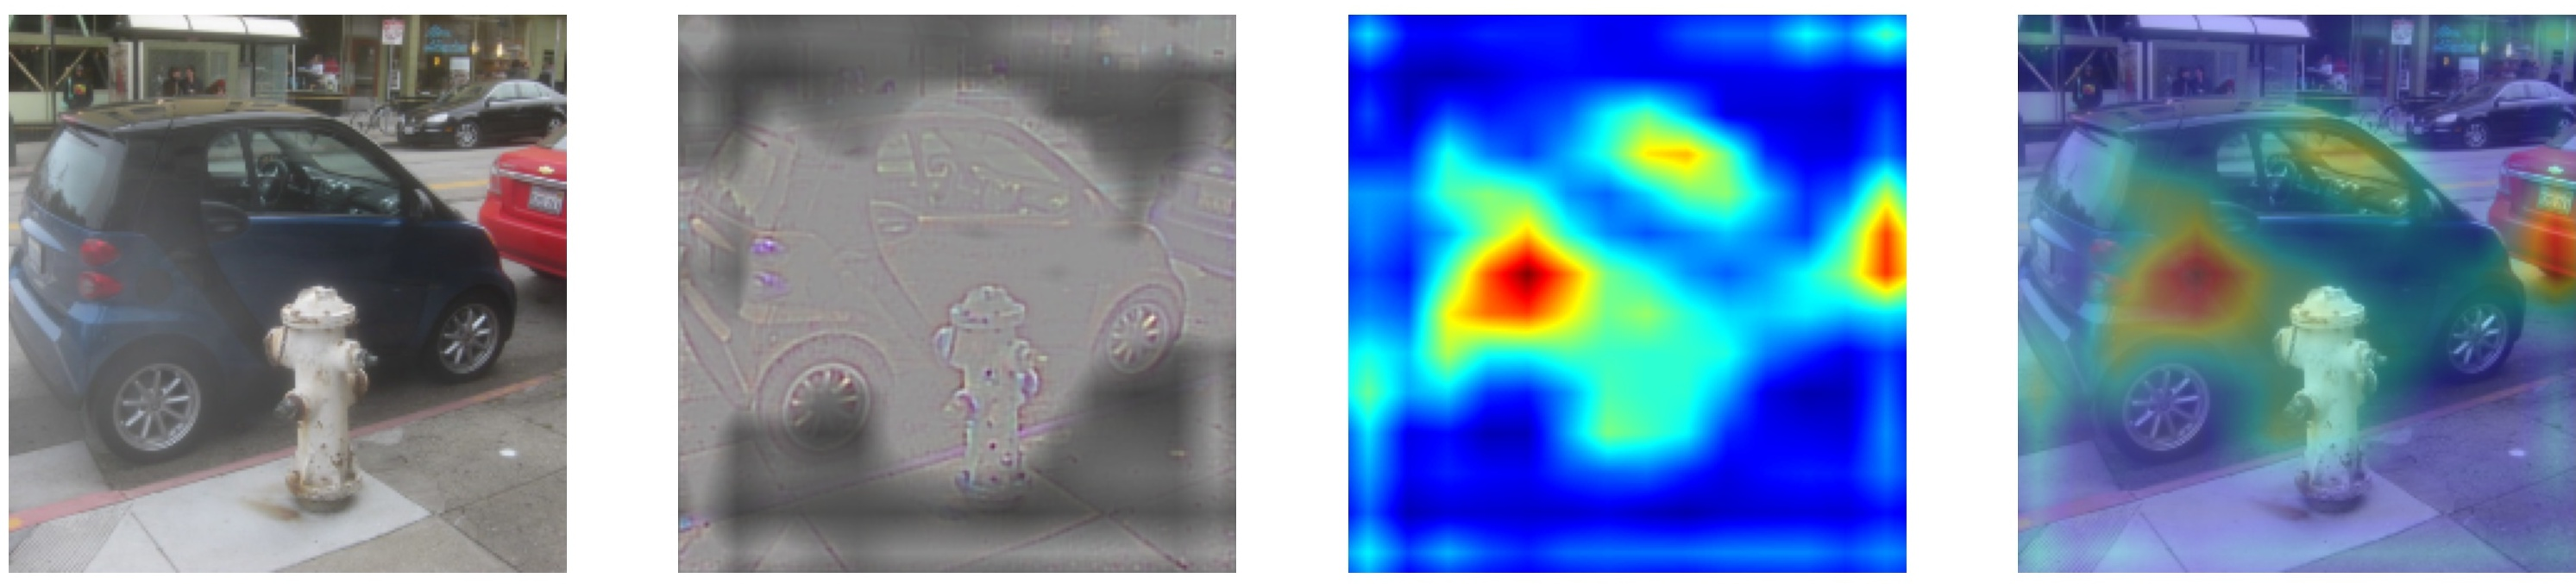
\includegraphics[width = \textwidth, height = 0.15\textwidth]{Images/HeatMapsPGD/out_test2.jpg}
     \end{subfigure}
    \begin{subfigure}{\textwidth}
        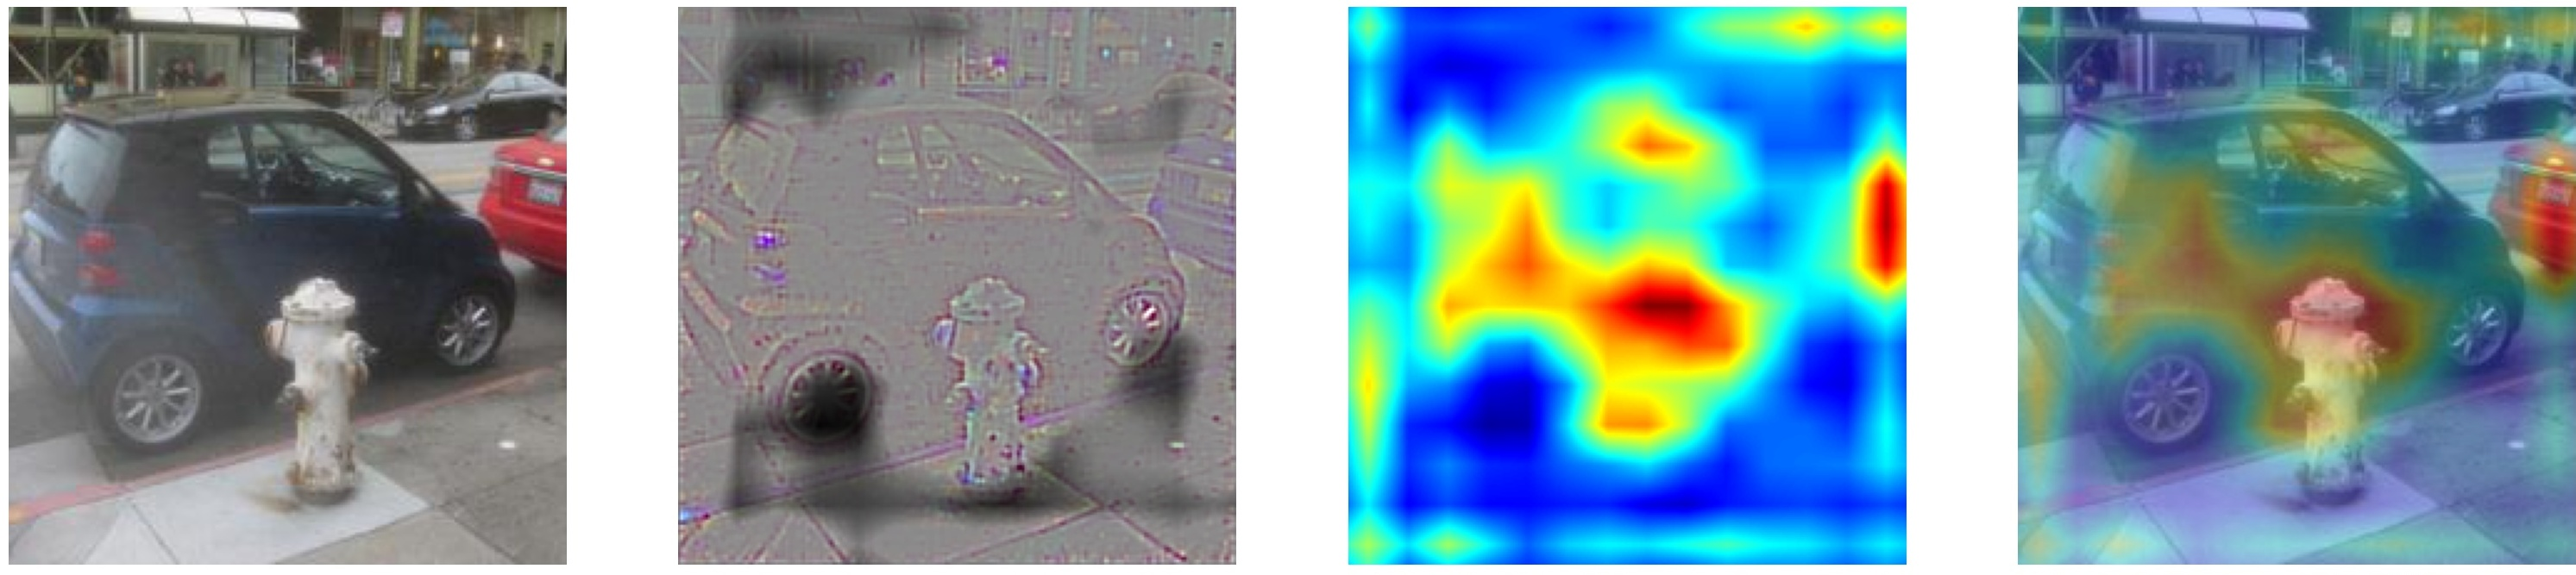
\includegraphics[width = \textwidth, height = 0.15\textwidth]{Images/HeatMapsPGD/out_att_test2.jpg}
    \end{subfigure}
    \begin{subfigure}{\textwidth}
        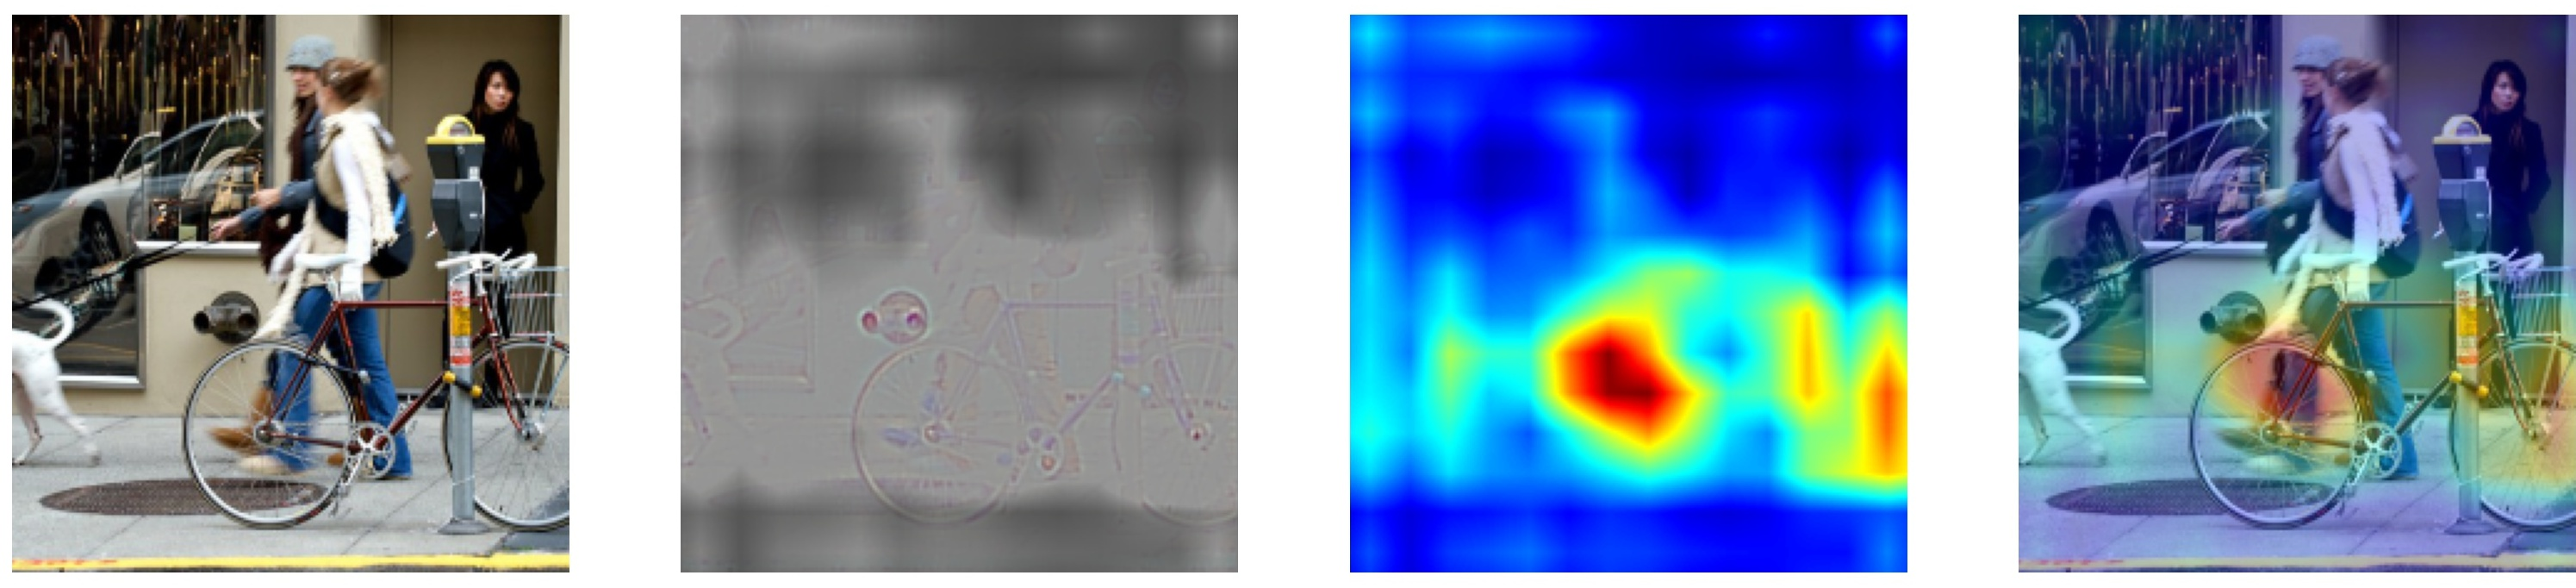
\includegraphics[width = \textwidth, height = 0.15\textwidth]{Images/HeatMapsPGD/out_test6.jpg}
     \end{subfigure}
    \begin{subfigure}{\textwidth}
        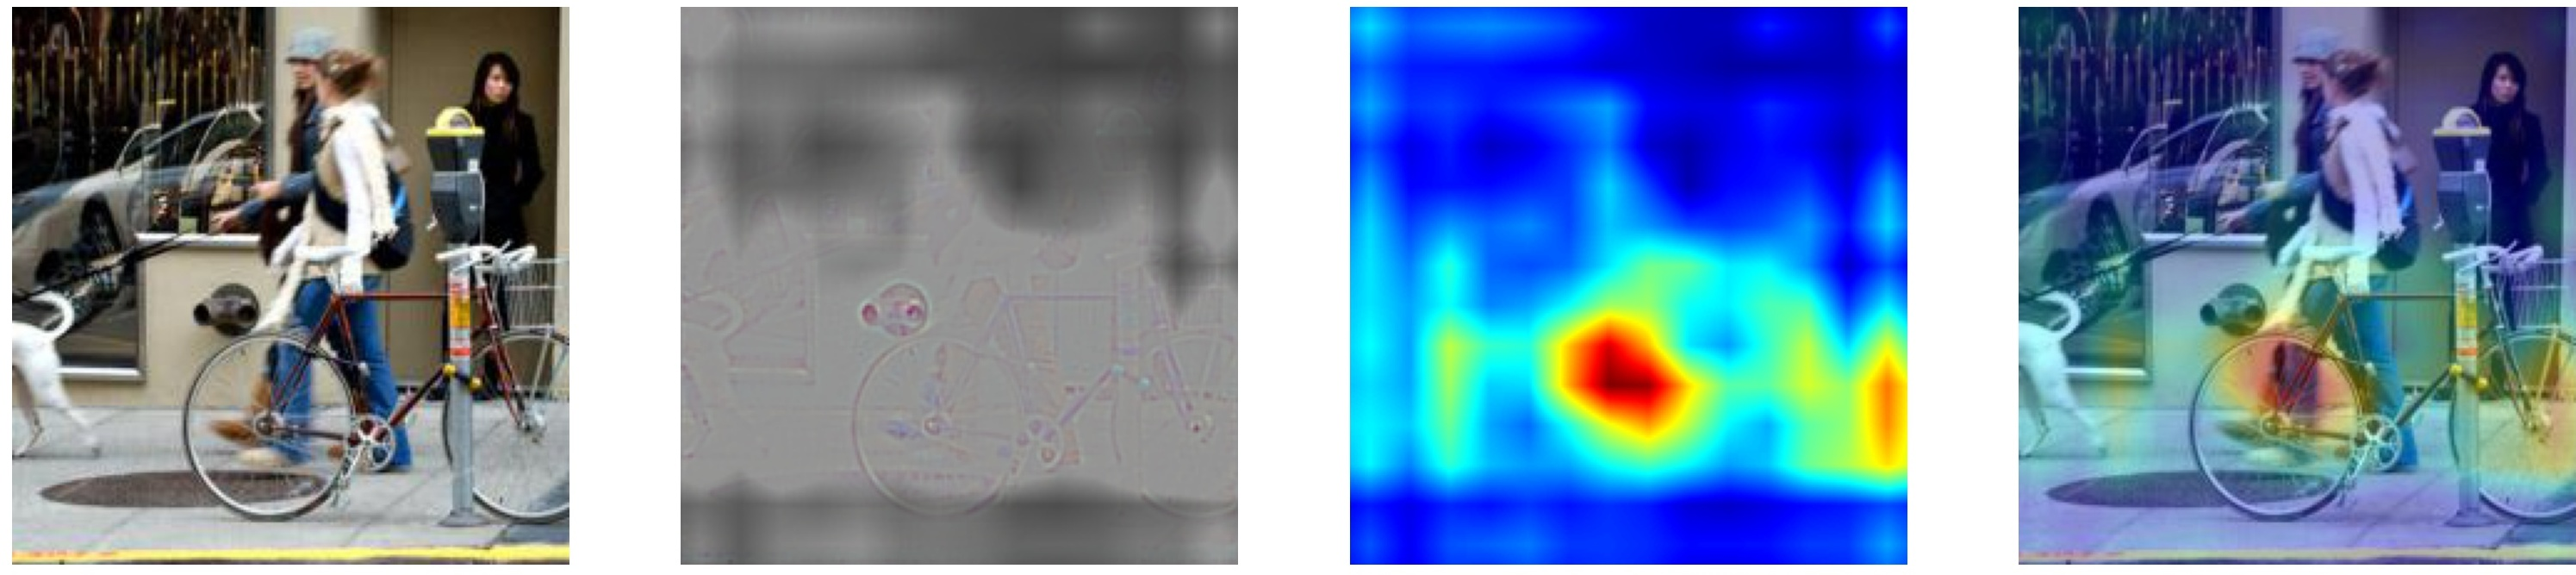
\includegraphics[width = \textwidth, height = 0.15\textwidth]{Images/HeatMapsPGD/out_att_test6.jpg}
    \end{subfigure}
    \begin{subfigure}{\textwidth}
        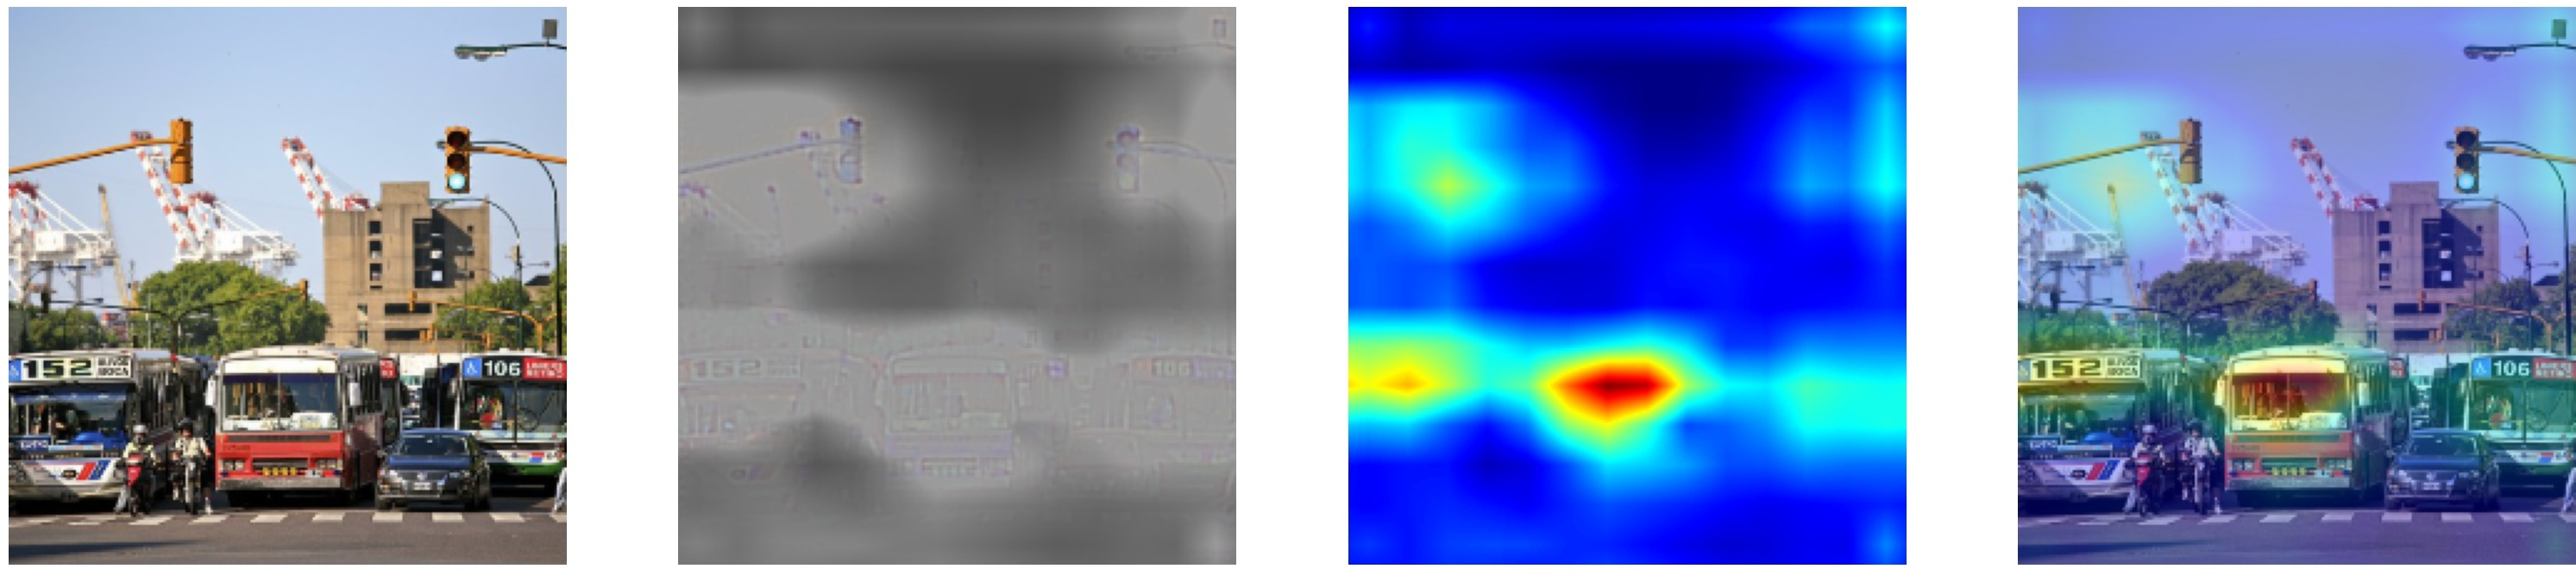
\includegraphics[width = \textwidth, height = 0.15\textwidth]{Images/HeatMapsPGD/out_test10.jpg}
     \end{subfigure}
    \begin{subfigure}{\textwidth}
        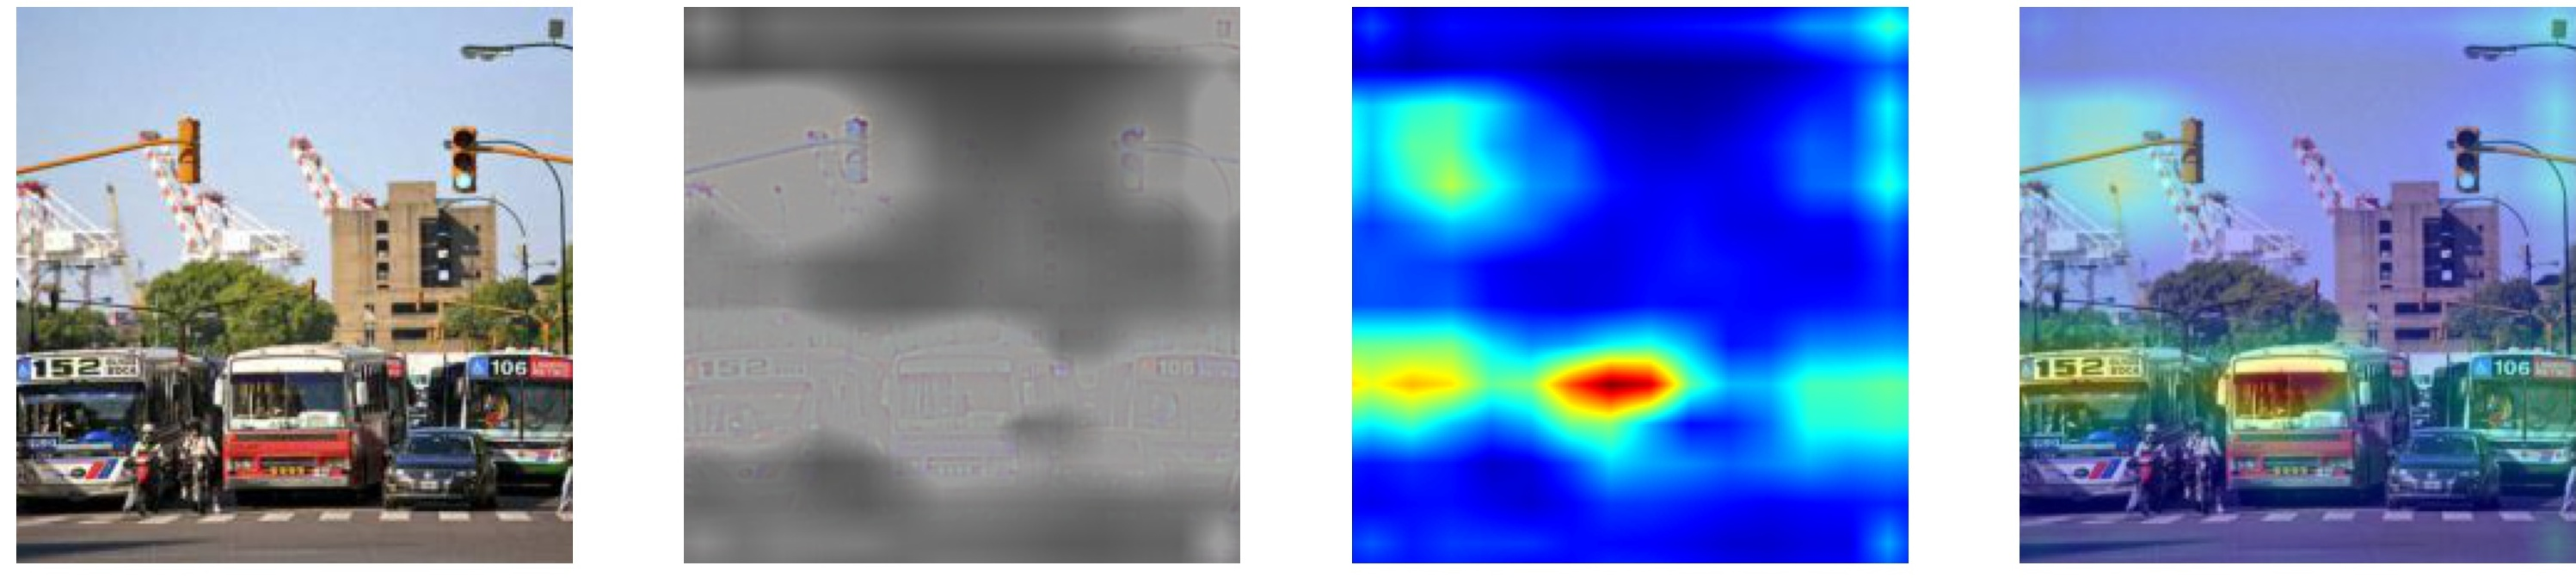
\includegraphics[width = \textwidth, height = 0.15\textwidth]{Images/HeatMapsPGD/out_att_test10.jpg}
    \end{subfigure}
    \caption{Heat maps generated by GradCAM++ on original and attacked images. In every pair, the first one is original and second one is attacked. }
    \label{fig:heat-PGD}
\end{figure*}
In order to come up with a more successful attack we started investigating which regions play crucial role in determining objectness and class scores in robust models like YOLO\emph{v3}. Towards this end, we started working on GradCAM++. But the problem with such techniques is they are engineered keeping in mind the general CNN architectures which are convolutional layers stacked upon fully connected layers and final layer gives out class conditional probabilities.\\
But architectures like Darknet (backbone of YOLO\emph{v3}) are not straight forward since they embed bounding box information into the layers, and predictions are given at various stages, moreover the structure of prediction is non trivial to infer analogy with formulations of GradCAM++.\\
An example prediction structure of YOLO\emph{v3} is shown in \figref{yolo-pred}(a) and architecture in \figref{yolo-pred}(b). An image goes through a series of residual blocks and down sampling is done through increasing stride. After reaching a fixed scale, we get a grid with information about bounding boxes stacked sequentially as shown in \figref{yolo-pred}(a). Then this grid is up sampled to go get two more predictions with different number of grid boxes as shown in \figref{yolo-pred}(b).\\
\begin{figure*}[h]
    \begin{subfigure}{0.35\textwidth}
        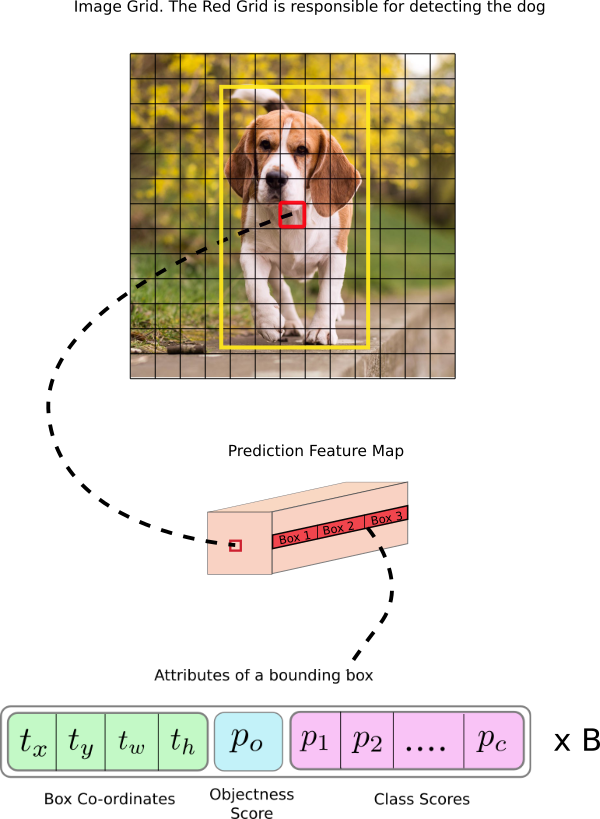
\includegraphics[width = \textwidth, height = \textwidth]{Images/Yolo-MS-COCO-Attacked/yolo-5.png}
    \end{subfigure}
    \begin{subfigure}{0.65\textwidth}
        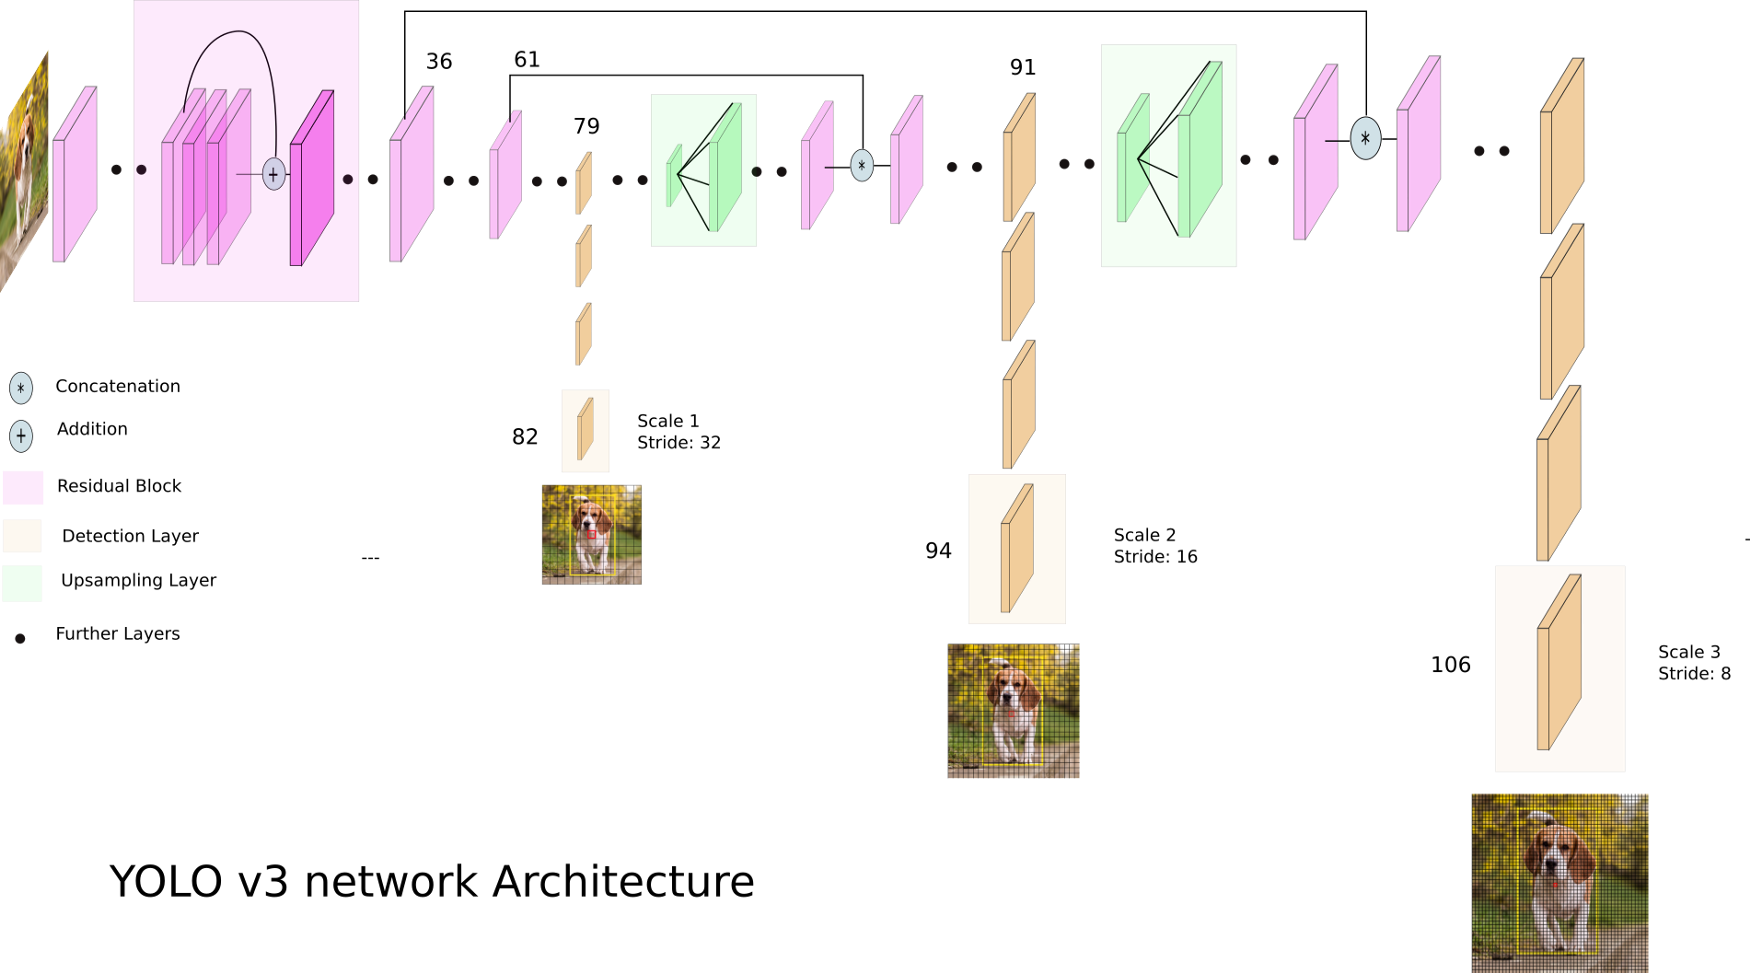
\includegraphics[width = \textwidth, height = \textwidth]{Images/yolov3-arch.png}
    \end{subfigure}
    \caption{(a) An example prediction from YOLO\emph{v3} on 13x13 grids \cite{kathuria_2019}. (b) Predictions from YOLO\emph{v3} \cite{kathuria_2018}.}
    \label{fig:yolo-pred}
\end{figure*}
Since our focus is on video data for autonomous driving, we studied how well GradCAM++ performs on the traffic symbols and we tried to answer the question: "Do we need to formulate a new approach for robust models like YOLO\emph{v3} or GradCAM++ is good enough to proceed?". To answer this we chose GSTRB\textsuperscript{\cite{Houben-IJCNN-2013}} dataset and trained VGG-16 model on it. Using this model, we generated heat maps for this dataset and result were satisfactory, as can be seen from \figref{heat-GSTRB}.\\
\begin{figure*}[h]
    \begin{subfigure}{\textwidth}
        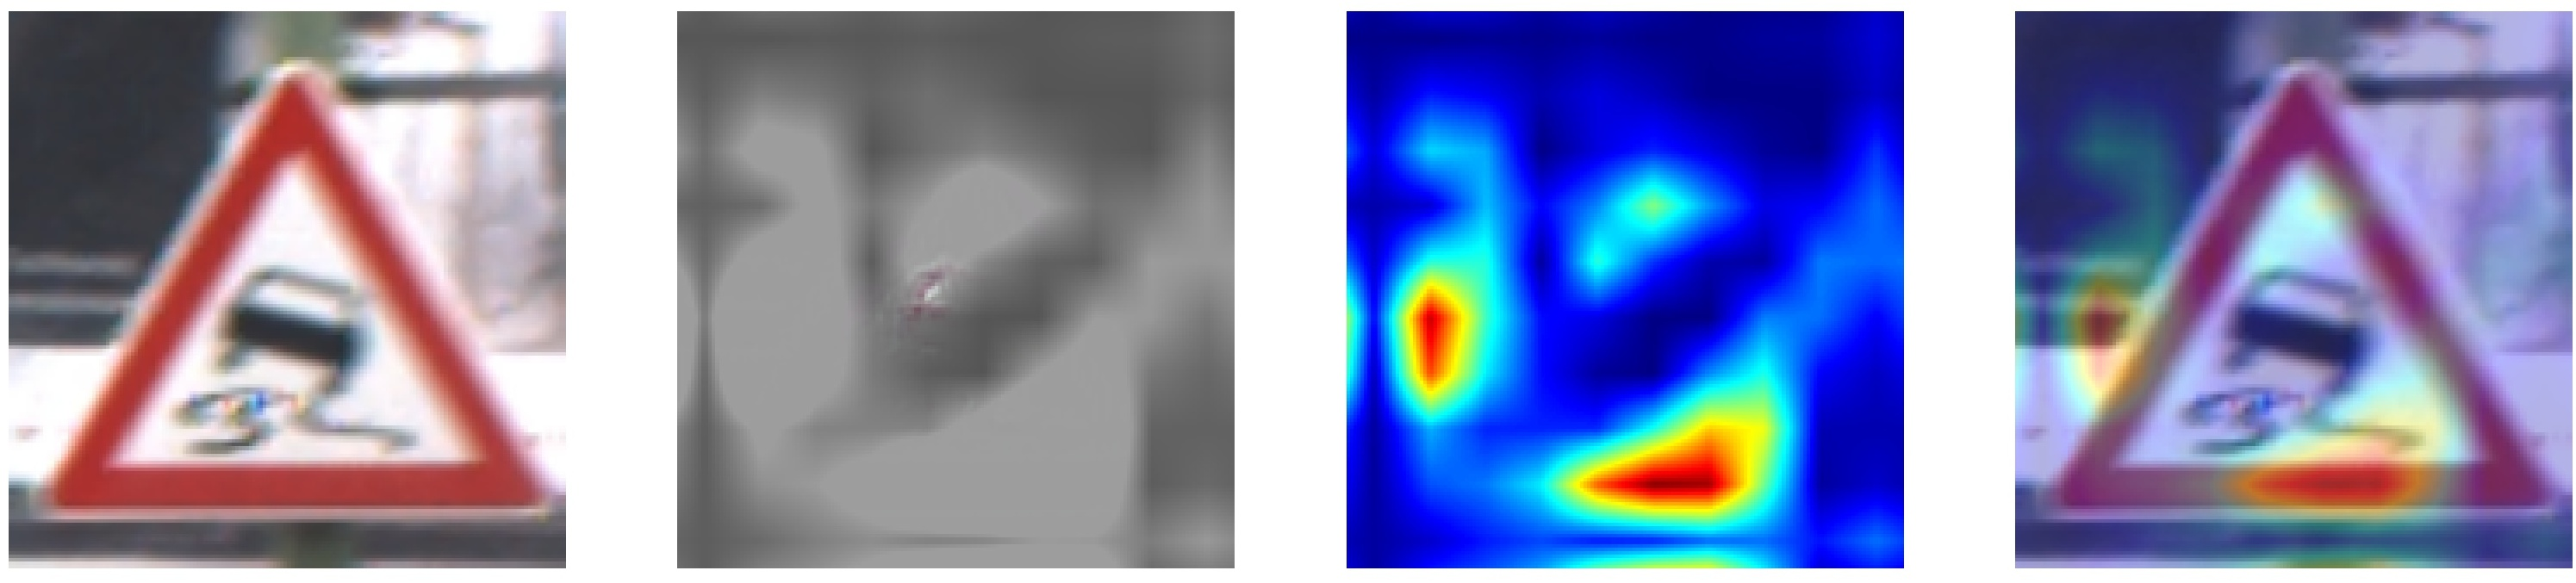
\includegraphics[width = \textwidth, height = 0.15\textwidth]{Images/GSTRB/16.jpg}
    \end{subfigure}
    \begin{subfigure}{\textwidth}
        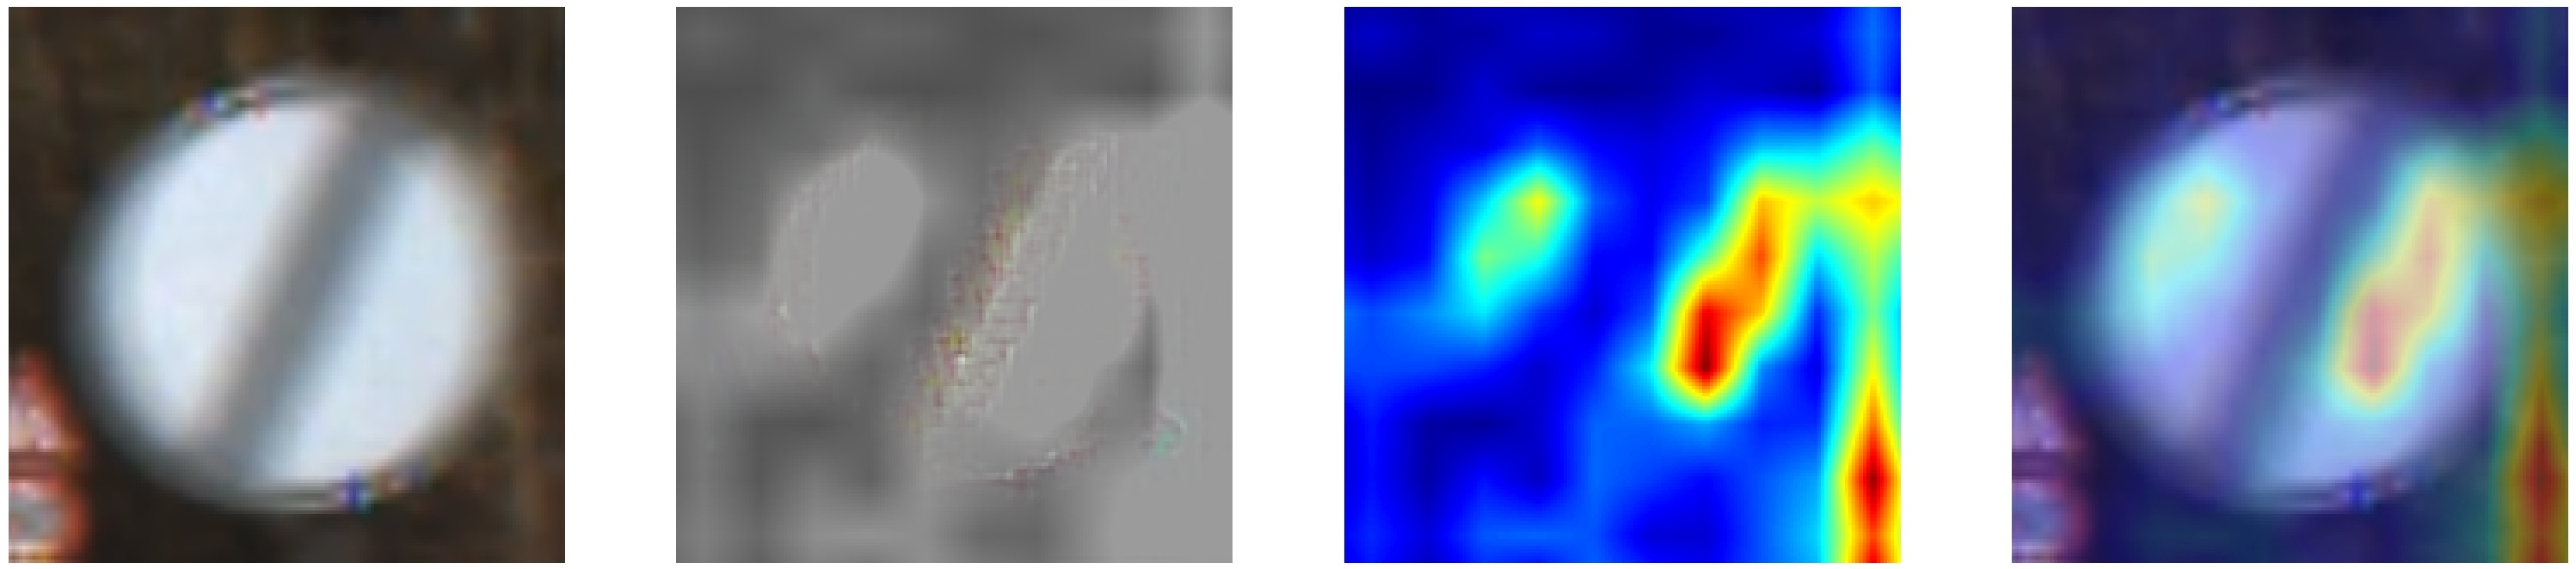
\includegraphics[width = \textwidth, height = 0.15\textwidth]{Images/GSTRB/17.jpg}
    \end{subfigure}
    \begin{subfigure}{\textwidth}
        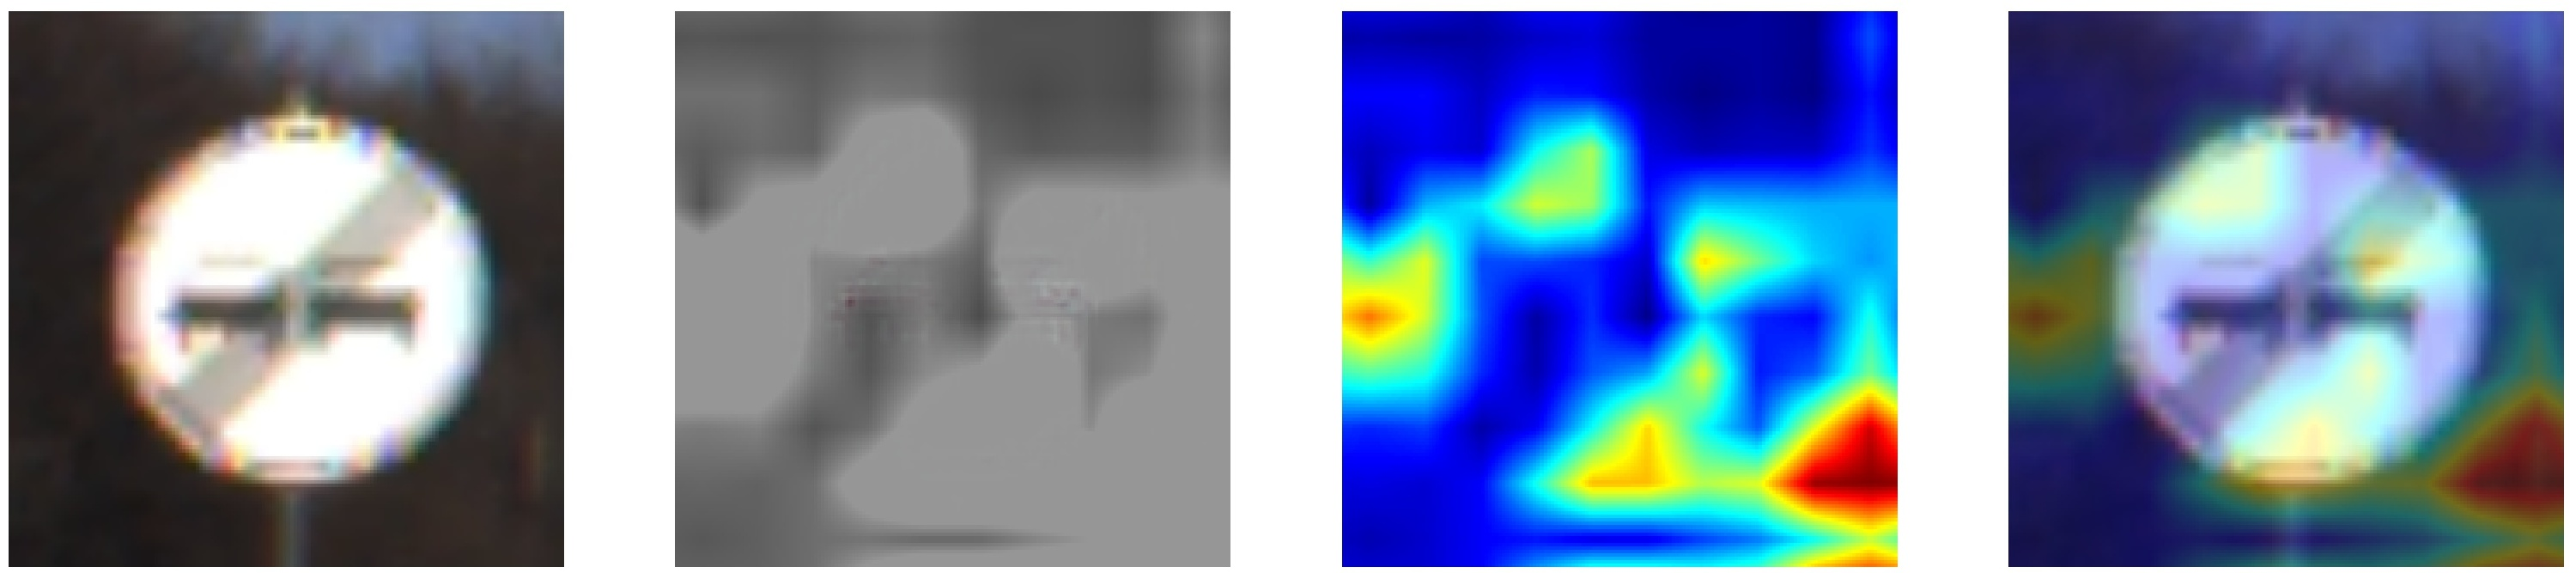
\includegraphics[width = \textwidth, height = 0.15\textwidth]{Images/GSTRB/20.jpg}
    \end{subfigure}
    \begin{subfigure}{\textwidth}
        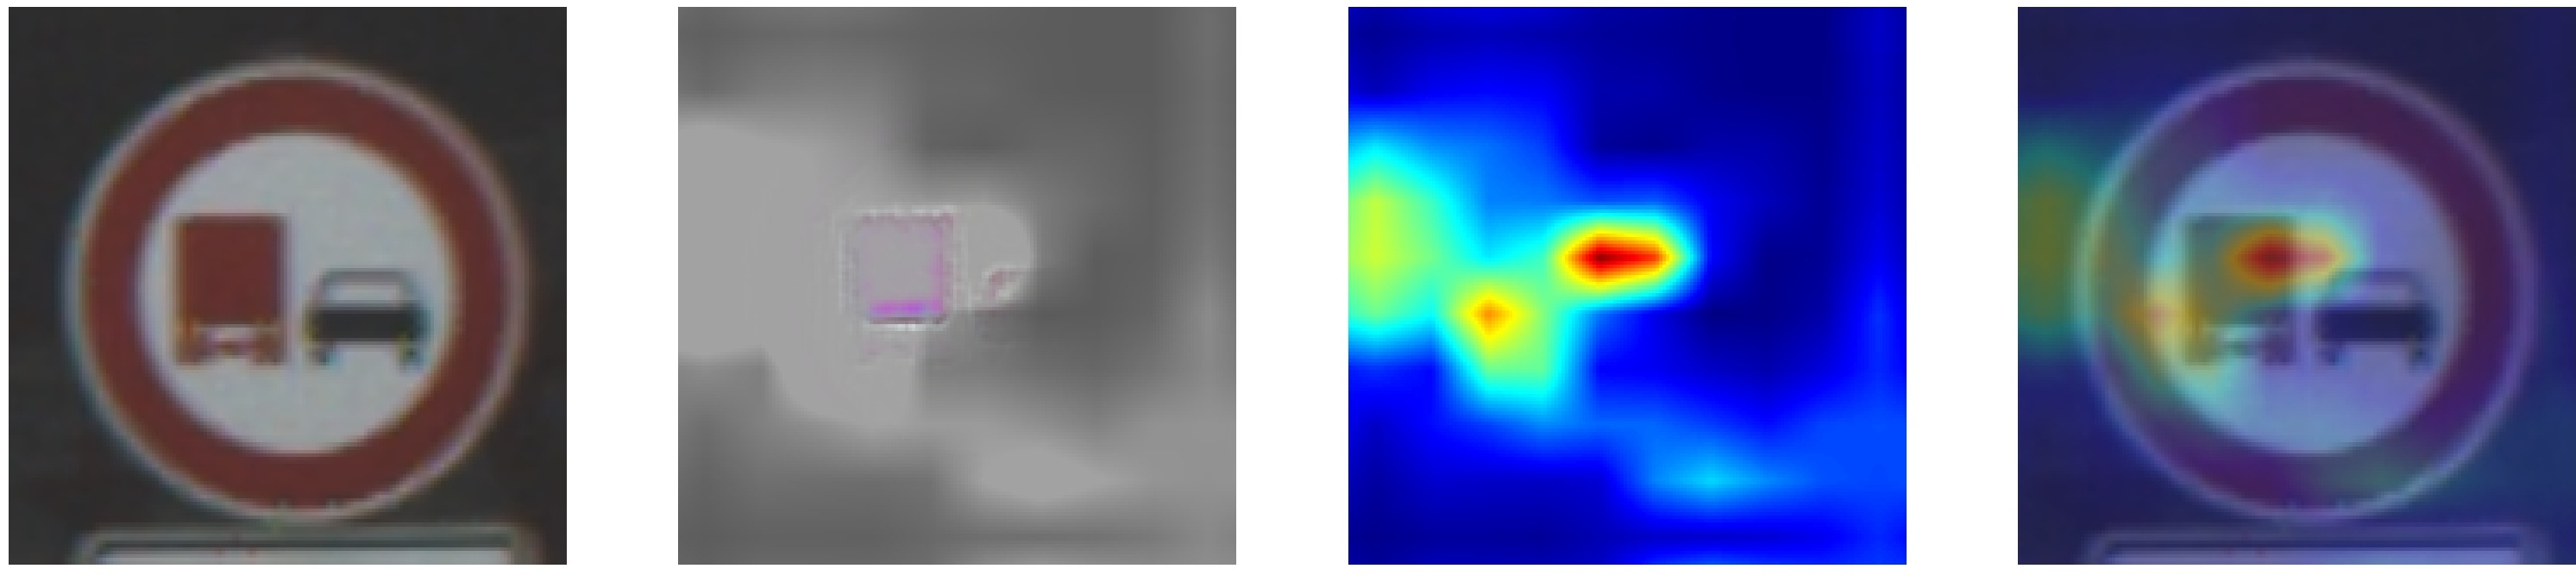
\includegraphics[width = \textwidth, height = 0.15\textwidth]{Images/GSTRB/4.jpg}
    \end{subfigure}
    \caption{Heat maps generated by GradCAM++ on GSTRB dataset.}
    \label{fig:heat-GSTRB}
\end{figure*}
Since GradCAM++ gives good visualizations for traffic signs and it also claimed to have good localization properties\textsuperscript{\cite{Chattopadhay_2018}} on mutli-object scenario, we studied how well these localized regoions can be leveraged with objectness score heat maps from YOLO\emph{v3}. To obtain the "objectness" heat maps from we used the object score channels of each anchor box for every grid. And then these scores were interpolated back to image to understand where exactly the model looks for object within the bounding box.\\
To conduct this experiment, we used CUB-2011\textsuperscript{\cite{WahCUB_200_2011}} dataset, with VGG-16 trained on ImageNet and YOLO\emph{v3} trained on MS-COCO dataset. The results include 2 images for each image input, where one of them signifies heat map from YOLO\emph{v3} as discussed above and the other one is GradCAM++ heatmap and both with the bounding box drawn onto the heat maps to understand their layout with respect to the localization by the non-max supressed bounding box of YOLO\emph{v3}. The results are shown in \figref{yolo-vgg}.\\
\begin{figure*}[h]
    \centering
    \begin{subfigure}{\textwidth}
        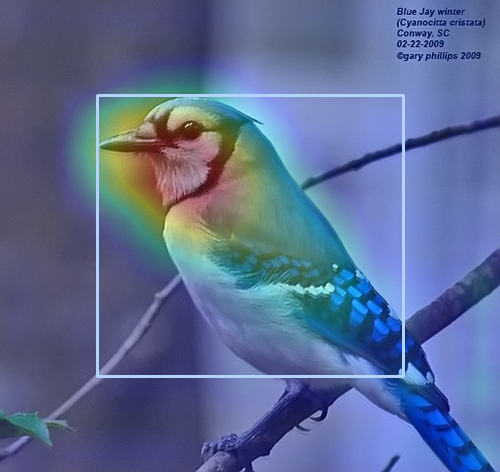
\includegraphics[width = 0.5\textwidth, height = 0.25\textwidth]{Images/CUB-VGG-Heat/new_vgg_bbox_heat_1.png}
        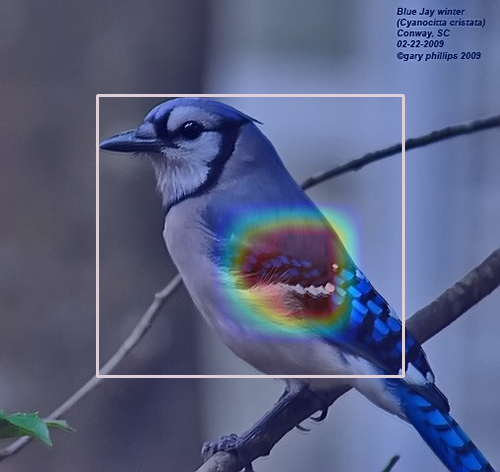
\includegraphics[width = 0.5\textwidth, height = 0.25\textwidth]{Images/CUB-YOLO-Heat/new_yolo_bbox_heat_0.png}
    \end{subfigure}
    \begin{subfigure}{\textwidth}
        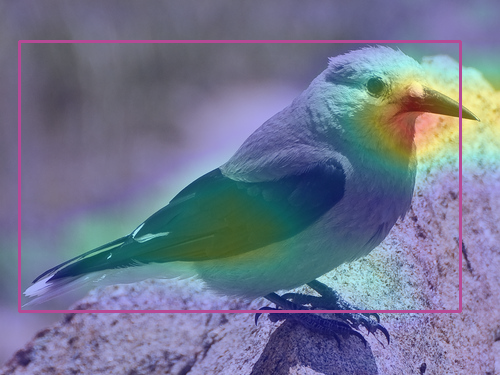
\includegraphics[width = 0.5\textwidth, height = 0.25\textwidth]{Images/CUB-VGG-Heat/new_vgg_bbox_heat_4.png}
        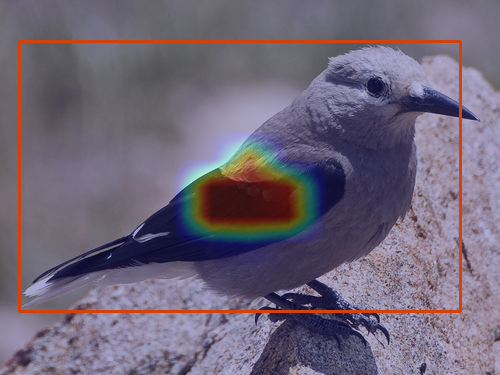
\includegraphics[width = 0.5\textwidth, height = 0.25\textwidth]{Images/CUB-YOLO-Heat/new_yolo_bbox_heat_4.png}
    \end{subfigure}
    \begin{subfigure}{\textwidth}
        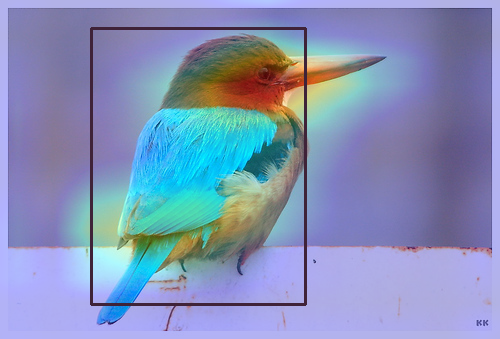
\includegraphics[width = 0.5\textwidth, height = 0.25\textwidth]{Images/CUB-VGG-Heat/new_vgg_bbox_heat_8.png}
        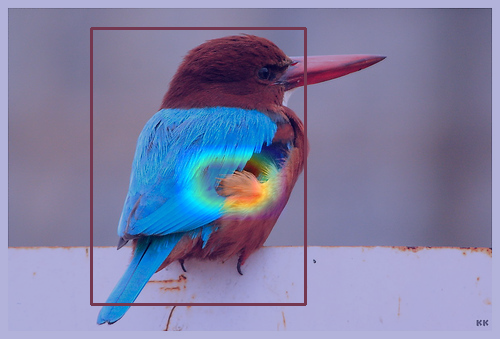
\includegraphics[width = 0.5\textwidth, height = 0.25\textwidth]{Images/CUB-YOLO-Heat/new_yolo_bbox_heat_8.png}
    \end{subfigure}
    \begin{subfigure}{\textwidth}
        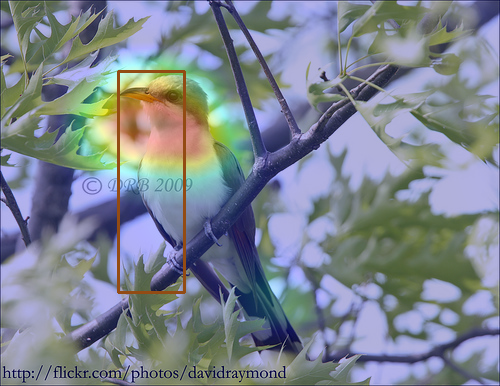
\includegraphics[width = 0.5\textwidth, height = 0.25\textwidth]{Images/CUB-VGG-Heat/new_vgg_bbox_heat_10.png}
        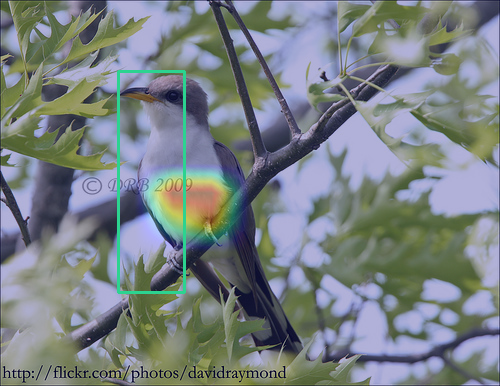
\includegraphics[width = 0.5\textwidth, height = 0.25\textwidth]{Images/CUB-YOLO-Heat/new_yolo_bbox_heat_10.png}
    \end{subfigure}
    \caption{YOLO\emph{v3} bounding boxes with heat maps generated through GradCAM++ and YOLO\emph{v3} objectness scores.}
    \label{fig:yolo-vgg}
\end{figure*}
As evident from the heat maps we need to combine these two aspects to detect more effective regions for attack purposes.\\
\section{Technologies and Resources}
Most of the architectures are implemented using PyTorch. Except GradCAM++, which uses TensorFlow. YOLO\emph{v3} is implemented from scratch\textsuperscript{\cite{kathuria_2019}} in PyTorch to extract "objectness" heat maps. The PGD attack is designed in PyTorch with reference to the tutorials\textsuperscript{\cite{madry}}. The VGG-16 nets on GSTRB and CUBD are trained locally using PyTorch. The GradCAm++ implementation is adopted from the paper itself, with modifications required on task-to-task basis.\\
Most of the computations are run locally on a system with Intel i7 processor, 8GB RAM, and Nvidia GeForce GTX 1050Ti.\\
\section{Results and Conclusion}
In conclusion, we can see that attacking datasets with simple attacks like PGD do not give satisfying success rates and we need to look deeper into regions of activation of the datasets with respect to robust models like YOLO\emph{v3}.\\
So in this direction, we contrasted how visualization techniques like GradCAM++, are specific for general CNNs and we need to come up with a hybrid approach which blends both GradCAM++ heat maps with YOLO\emph{v3}'s objectness heat maps to come with finer and feasible regions for attacks.\\
\section{Future Work}
We are thinking of extending this approach and devise new formulation for architectures like YOLO\emph{v3} and utilize these mappings to create noise patches that could fool the object detectors.
\printbibliography
\end{document}